\documentclass[10pt]{article}
\usepackage[margin=1in]{geometry}
\usepackage{amsmath,amssymb,booktabs,graphicx,microtype}
\usepackage[font=small,labelfont=bf]{caption}
\usepackage[colorlinks=true,allcolors=blue!60!black]{hyperref}

\title{Vessel-GNC: a compact C++/Python laboratory for\\simulation, estimation and optimal control of autonomous surface vessels}
\author{Charles Dhainaut}
\date{}

\begin{document}
\maketitle

\begin{abstract}
This note documents \texttt{vessel-gnc}, a compact simulation, estimation
and control stack for autonomous surface vessels. A 3-DOF horizontal-plane
model (Fossen-style) is integrated by a C++20 kernel and, independently, by
a symbolic CasADi predictor; the two are cross-validated to $10^{-8}$ on
every test run. Around this kernel sit an extended Kalman filter with an
augmented current-equivalent state, classical LOS/PID baselines, a
disturbance-aware nonlinear MPC and a geometric model predictive contouring
controller. Four controllers are compared on one flagship scenario (a
200\,m S-curve under rotating current and wind gusts, with noisy sensors
and a perturbed truth plant): RMS cross-track error falls from
$0.69$\,m (LOS) to $0.23$\,m (disturbance-aware NMPC). Every number quoted
here is regenerated from committed JSON artifacts by one tool, and a
determinism check replays the whole scenario against them. What the
project validates is the numerics and the control chain; the physical
parameters are illustrative and are not fitted to a real hull.
\end{abstract}

\section{Introduction}
Autonomous-vessel guidance work usually falls into one of two camps: a
flight-stack style autopilot, where the model is buried under hardware
abstraction, or a research codebase, where the model is explicit but the
engineering is thin. \texttt{vessel-gnc} sits deliberately in between. It
is small enough to read in an afternoon, but it is built like instrument
software: deterministic by default, cross-validated where two
implementations of the same physics meet, and honest about what is
verified, what is validated, and what is merely illustrative.

The chain is the one that matters in practice:
\begin{equation}
  \text{plant} \;\rightarrow\; \text{sensors} \;\rightarrow\;
  \text{estimator} \;\rightarrow\; \text{controller} \;\rightarrow\;
  \text{actuators},
\end{equation}
run closed-loop, with the controller never seeing the true state or the
true environment. The sections below walk through each block, then the
measured comparison of four controllers, and finally the reproducibility
contract that keeps the published numbers honest.

\section{Vessel model}
\label{sec:model}
\paragraph{Frames and state.}
Positions and headings are inertial North--East, with $\psi$ clockwise from
North (equivalently a $z$-down convention); body axes are $x$ forward
(surge), $y$ starboard (sway). The pose and body velocity are
$\eta=[x,y,\psi]^\mathsf{T}$ and $\nu=[u,v,r]^\mathsf{T}$, with
\begin{equation}
  \dot\eta = R(\psi)\,\nu, \qquad
  R(\psi)=
  \begin{bmatrix}
    \cos\psi & -\sin\psi \\
    \sin\psi & \cos\psi
  \end{bmatrix}.
\end{equation}

\paragraph{Hydrodynamics.}
The momentum equation is written on the velocity \emph{relative} to the
water,
\begin{equation}
  \label{eq:momentum}
  M\dot\nu + C(\nu_{\mathrm{rel}})\,\nu_{\mathrm{rel}}
  + D(\nu_{\mathrm{rel}})\,\nu_{\mathrm{rel}}
  = \tau + \tau_{\mathrm{env}} + \dot\nu_c^{\,b},
\end{equation}
with the diagonal mass matrix
$M=\mathrm{diag}(m+X_{\dot u},\, m+Y_{\dot v},\, I_z+N_{\dot r})$ and the
skew-symmetric Coriolis form for diagonal $M$,
\begin{equation}
  C(\nu_{\mathrm{rel}})\,\nu_{\mathrm{rel}} =
  \begin{bmatrix}
    -m_{22}\,v_{\mathrm{rel}}\,r \\
    \phantom{-}m_{11}\,u_{\mathrm{rel}}\,r \\
    (m_{22}-m_{11})\,u_{\mathrm{rel}}\,v_{\mathrm{rel}}
  \end{bmatrix}.
\end{equation}
The yaw component is the destabilizing Munk coupling: for a slender hull
($m_{22}>m_{11}$) it assists a turn once the vessel develops sideslip. It
is kept on purpose, and the default parameters leave yaw damping dominant
at cruise so the vessel is directionally stable. Damping is linear plus
quadratic in the relative velocity,
$X_u u_r + X_{|u|u}|u_r|u_r$ per axis.

The current is a quasi-static spatial field: at each instant the flow
around the hull is treated as locally uniform and irrotational, so
Eq.~\eqref{eq:momentum} is unchanged and the field is simply sampled at
the vessel position. The flagship scenario places a Rankine eddy (a
solid-body core of 35\,m radius with irrotational $1/r$ decay outside) on
top of a slowly rotating base flow. Because the body frame rotates under a
turning vessel, a current that is inertially constant gains a transport
acceleration in body coordinates,
\begin{equation}
  \dot\nu_c^{\,b} = -S(r)\,v_c^{\,b}
  = \bigl(r\,v_c,\; -r\,u_c,\; 0\bigr)^\mathsf{T}.
\end{equation}
This term is small, easy to forget, and exactly the kind of detail the
cross-validation tests exist for (Sect.~\ref{sec:kernel}). Wind is a
constant inertial force rotated into the body frame.

\paragraph{Actuators.}
Commanded forces are not applied directly. Each channel is a rate-limited
first-order response with a smooth saturation model (docs/model.md
gives the derivation):
\begin{equation}
  \dot T = \dot T_{\max}\tanh\!\left(
    \frac{\mathrm{clamp}(T_{\mathrm{cmd}}) - T}{\tau_T\,\dot T_{\max}}
  \right),
\end{equation}
which keeps $|\dot T| < \dot T_{\max}$ exactly, is $C^1$ (good for
gradient-based solvers), and reduces to a plain lag for small errors. The
state is projected back into the physical bounds after every step.

\section{Simulation kernel and cross-validation}
\label{sec:kernel}
The C++20 kernel owns the plant: kinematics, hydrodynamics, actuator and a
fixed-step RK4 integrator, exposed to Python through pybind11. The
controllers need symbolic dynamics, so the predictor is a \emph{second},
independent implementation of Eqs.~\eqref{eq:momentum} in CasADi, with the
8-state (vessel + actuator) composition matching the kernel step for step:
actuator first, then the vessel with the resulting forces held constant.

These two implementations are tested against each other over random states
with non-zero current and wind, including out-of-bound actuator states and
out-of-range commands; agreement is better than $10^{-8}$. This is the
cheap insurance that pays for itself whenever either side changes.

\section{State estimation}
The filter is an extended Kalman filter over
$x=[\eta,\nu,c_N,c_E]$, where the last two components are an
\emph{equivalent-current} velocity. The augmented state is a proxy: under
combined uncertainty (wind plus model mismatch) it absorbs whatever
low-frequency velocity the model cannot explain. That is a feature, not a
bug, and the flag is made explicit in the reports.

Sensors (GNSS position, compass, gyro, speed log) are sampled
asynchronously with Gaussian noise, seeded, and delivered at their own
rates. The prediction uses the nominal plant: the same RK4 kernel as the
simulator, with the \emph{estimated} current as the relative-velocity
reference. The update is a linear observation of state components, applied
in Joseph form with explicit symmetrization. Figure~\ref{fig:estimation}
shows the equivalent-current state in the flagship scenario: it converges
toward the physical current, and the residual is the wind/model part it
was never meant to separate.

\begin{figure}[t]
  \centering
  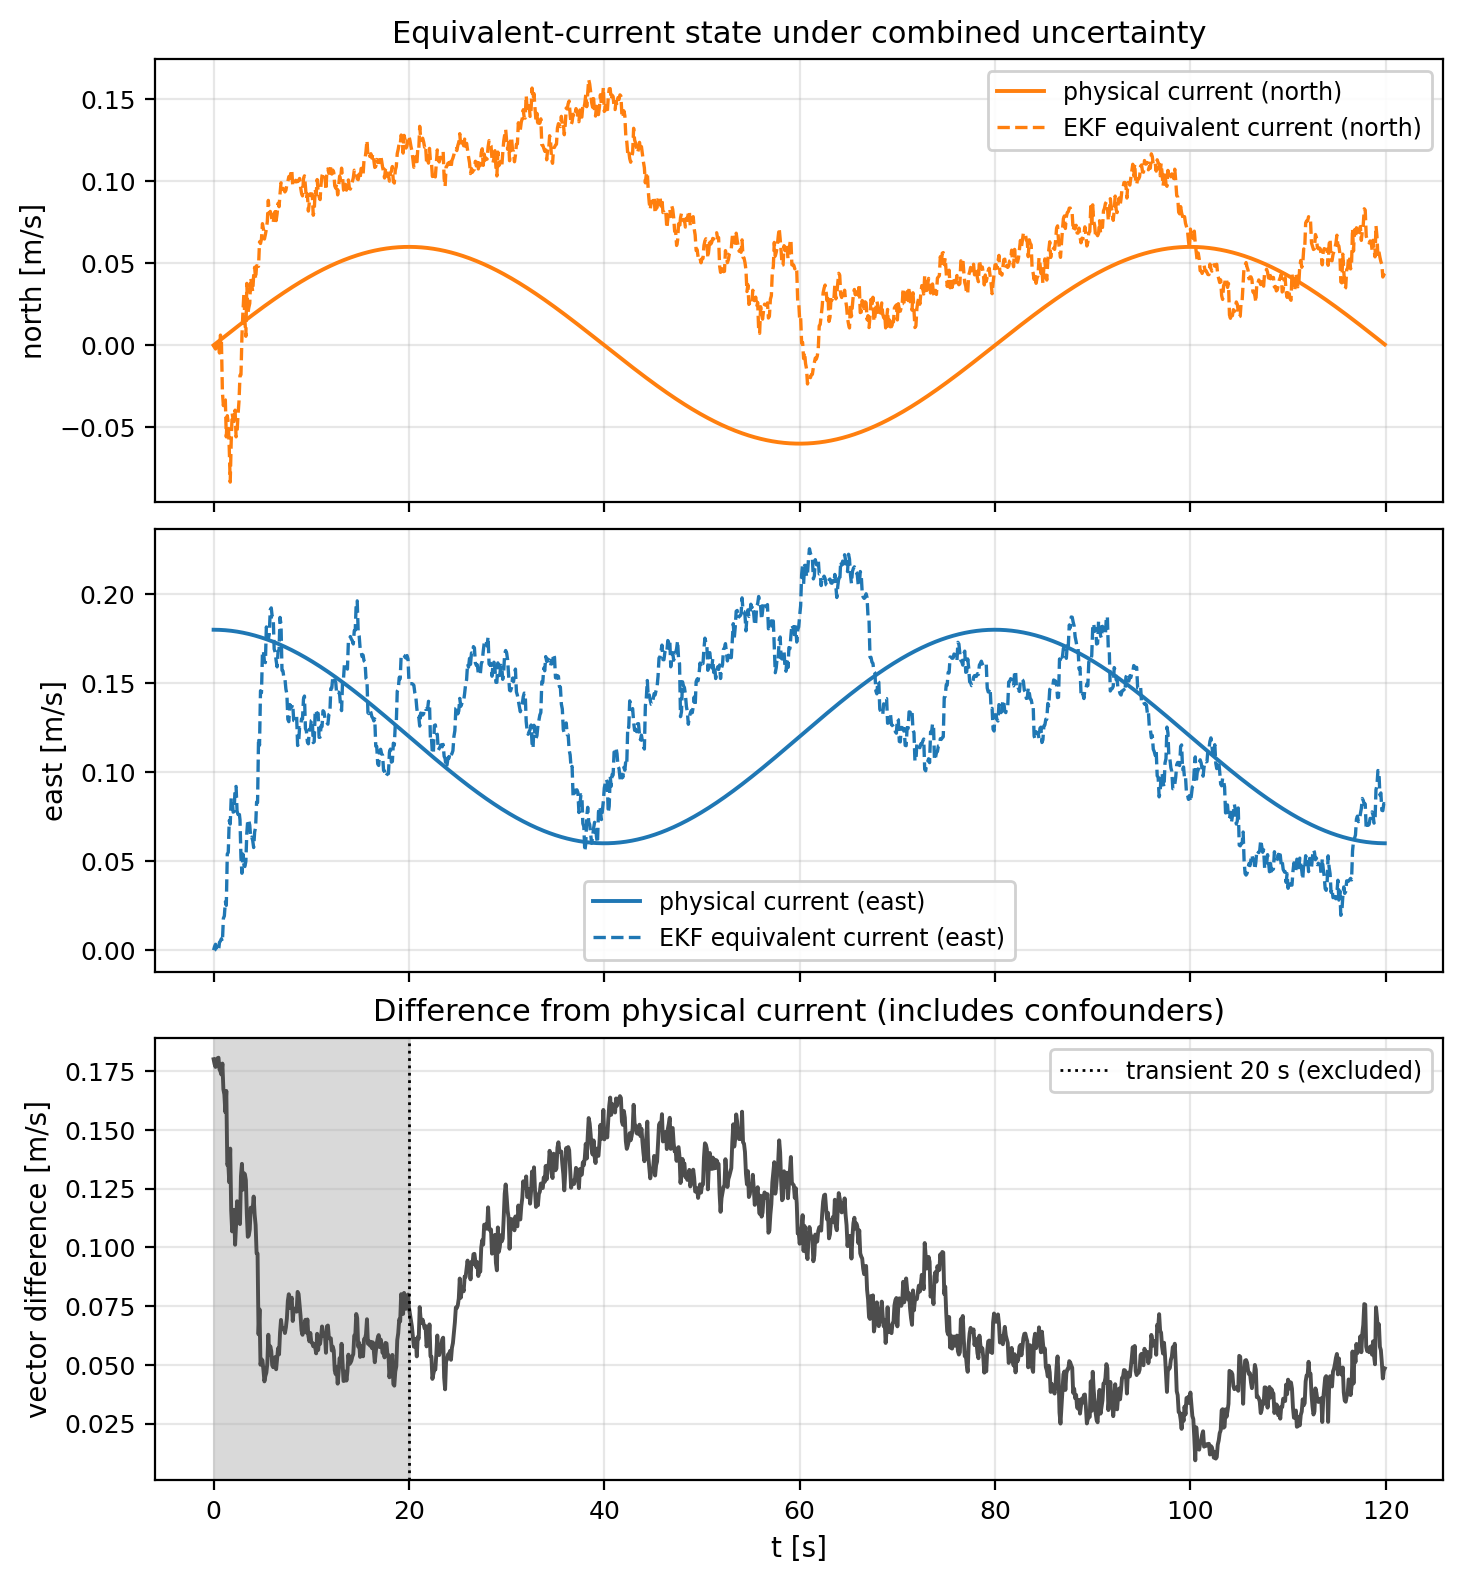
\includegraphics[width=0.62\textwidth]{figs/current_estimation.png}
  \caption{Physical current and EKF equivalent-current state in the
  combined-uncertainty flagship run. The difference (bottom) is dominated
  by gusts and model mismatch; it is not a current-sensor error.}
  \label{fig:estimation}
\end{figure}

\section{Controllers}
Four controllers share the same estimator output and the same actuator
model.

\paragraph{LOS + PID/PI.}
The classical baseline: a lookahead point at 8\,m drives the desired
heading, tracked by a PID on the wrapped heading error (derivative on the
measurement, conditional anti-windup), with a PI speed loop.

\paragraph{Nonlinear MPC.}
A discrete-time OCP over a 10\,s horizon ($N=25$, $t_s=0.4$\,s, two RK4
sub-steps per step),
\begin{equation}
  \min \sum_{k=0}^{N-1}
  q_p\lVert p_k - p_k^{\mathrm{ref}}\rVert^2
  + q_\psi e_{\psi,k}^2
  + r\,\Delta u_k^2 + s\,u_k^2,
\end{equation}
subject to the 8-state predictor and hard actuator bounds, solved with
IPOPT through CasADi at 5\,Hz, warm-started from the previous solution
shifted by one step. Termination is iteration- and tolerance-based
($\mathrm{tol}=10^{-4}$); there is deliberately no wall-clock cut, which
would make accepted iterates depend on machine load.

\paragraph{Disturbance-aware NMPC.}
The same OCP, but the current-equivalent estimate enters the predictor and
is held constant over the horizon. The controller does not get the true
environment; it gets the filter's guess.

\paragraph{Geometric MPCC.}
The fourth controller drops the mission clock entirely and follows the
path geometry: a monotone chord-progress state $s$ is driven by a bounded
virtual speed $V_s$, and the cost trades contouring and lag errors,
\begin{equation}
  e_c = t_\perp^\mathsf{T}(p - p(s)), \qquad
  e_l = t^\mathsf{T}(p - p(s)),
\end{equation}
against heading error and progress reward. A small quadratic term on
$V_s$ ($r_{vs}=0.5$) keeps the corresponding Hessian block positive
definite; without it IPOPT stalls on the first S-curve turn. Failed solves
are never applied: the fallback is the previously commanded action.

\section{Results}
\label{sec:results}
The flagship scenario is one smooth S-curve (200.087\,m chord progress),
120\,s at $t=0.01$\,s, seed 42. The plant uses \emph{perturbed} truth
parameters ($+10\%$ mass, $+15\%$ inertia, reduced damping) behind a
rate-limited actuator; the environment is a rotating base current, a
Rankine eddy and two wind gusts; the sensors are noisy and asynchronous.
Controllers see only the EKF output. The operational requirement is a
$\pm 1$\,m corridor around the reference: the LOS baseline violates it
(max cross-track 1.07\,m), while all three predictive controllers hold
it. Table~\ref{tab:metrics} is generated from the committed artifacts;
Fig.~\ref{fig:comparison} shows the same comparison in time domain.

\begin{table}[h]
\centering
\small
\begin{tabular}{lcccc}
\toprule
& LOS & Nominal NMPC & Aware NMPC & MPCC \\
\midrule
RMS cross-track $[\mathrm{m}]$      & 0.69 & 0.41 & \textbf{0.23} & 0.25 \\
P95 cross-track $[\mathrm{m}]$      & 0.98 & 0.65 & 0.53 & 0.61 \\
Max cross-track $[\mathrm{m}]$      & 1.07 & 0.74 & 0.63 & 0.71 \\
RMS heading error $[\mathrm{deg}]$  & 7.1 & 10.5 & 11.2 & 9.8 \\
Final path progress $[\mathrm{m}]$  & 154.9 & 156.2 & 156.1 & \textbf{164.2} \\
RMS thrust $[\mathrm{N}]$           & 31.8 & 33.7 & 33.5 & 36.6 \\
Either channel saturated $[\mathrm{s}]$ & 0.0 & 2.5 & 1.7 & 2.3 \\
\bottomrule
\end{tabular}
\caption{Deterministic flagship metrics (120\,s, seed 42). The
disturbance-aware NMPC halves the LOS tracking error; MPCC buys progress
at the cost of actuator effort.}
\label{tab:metrics}
\end{table}

\begin{figure}[t]
  \centering
  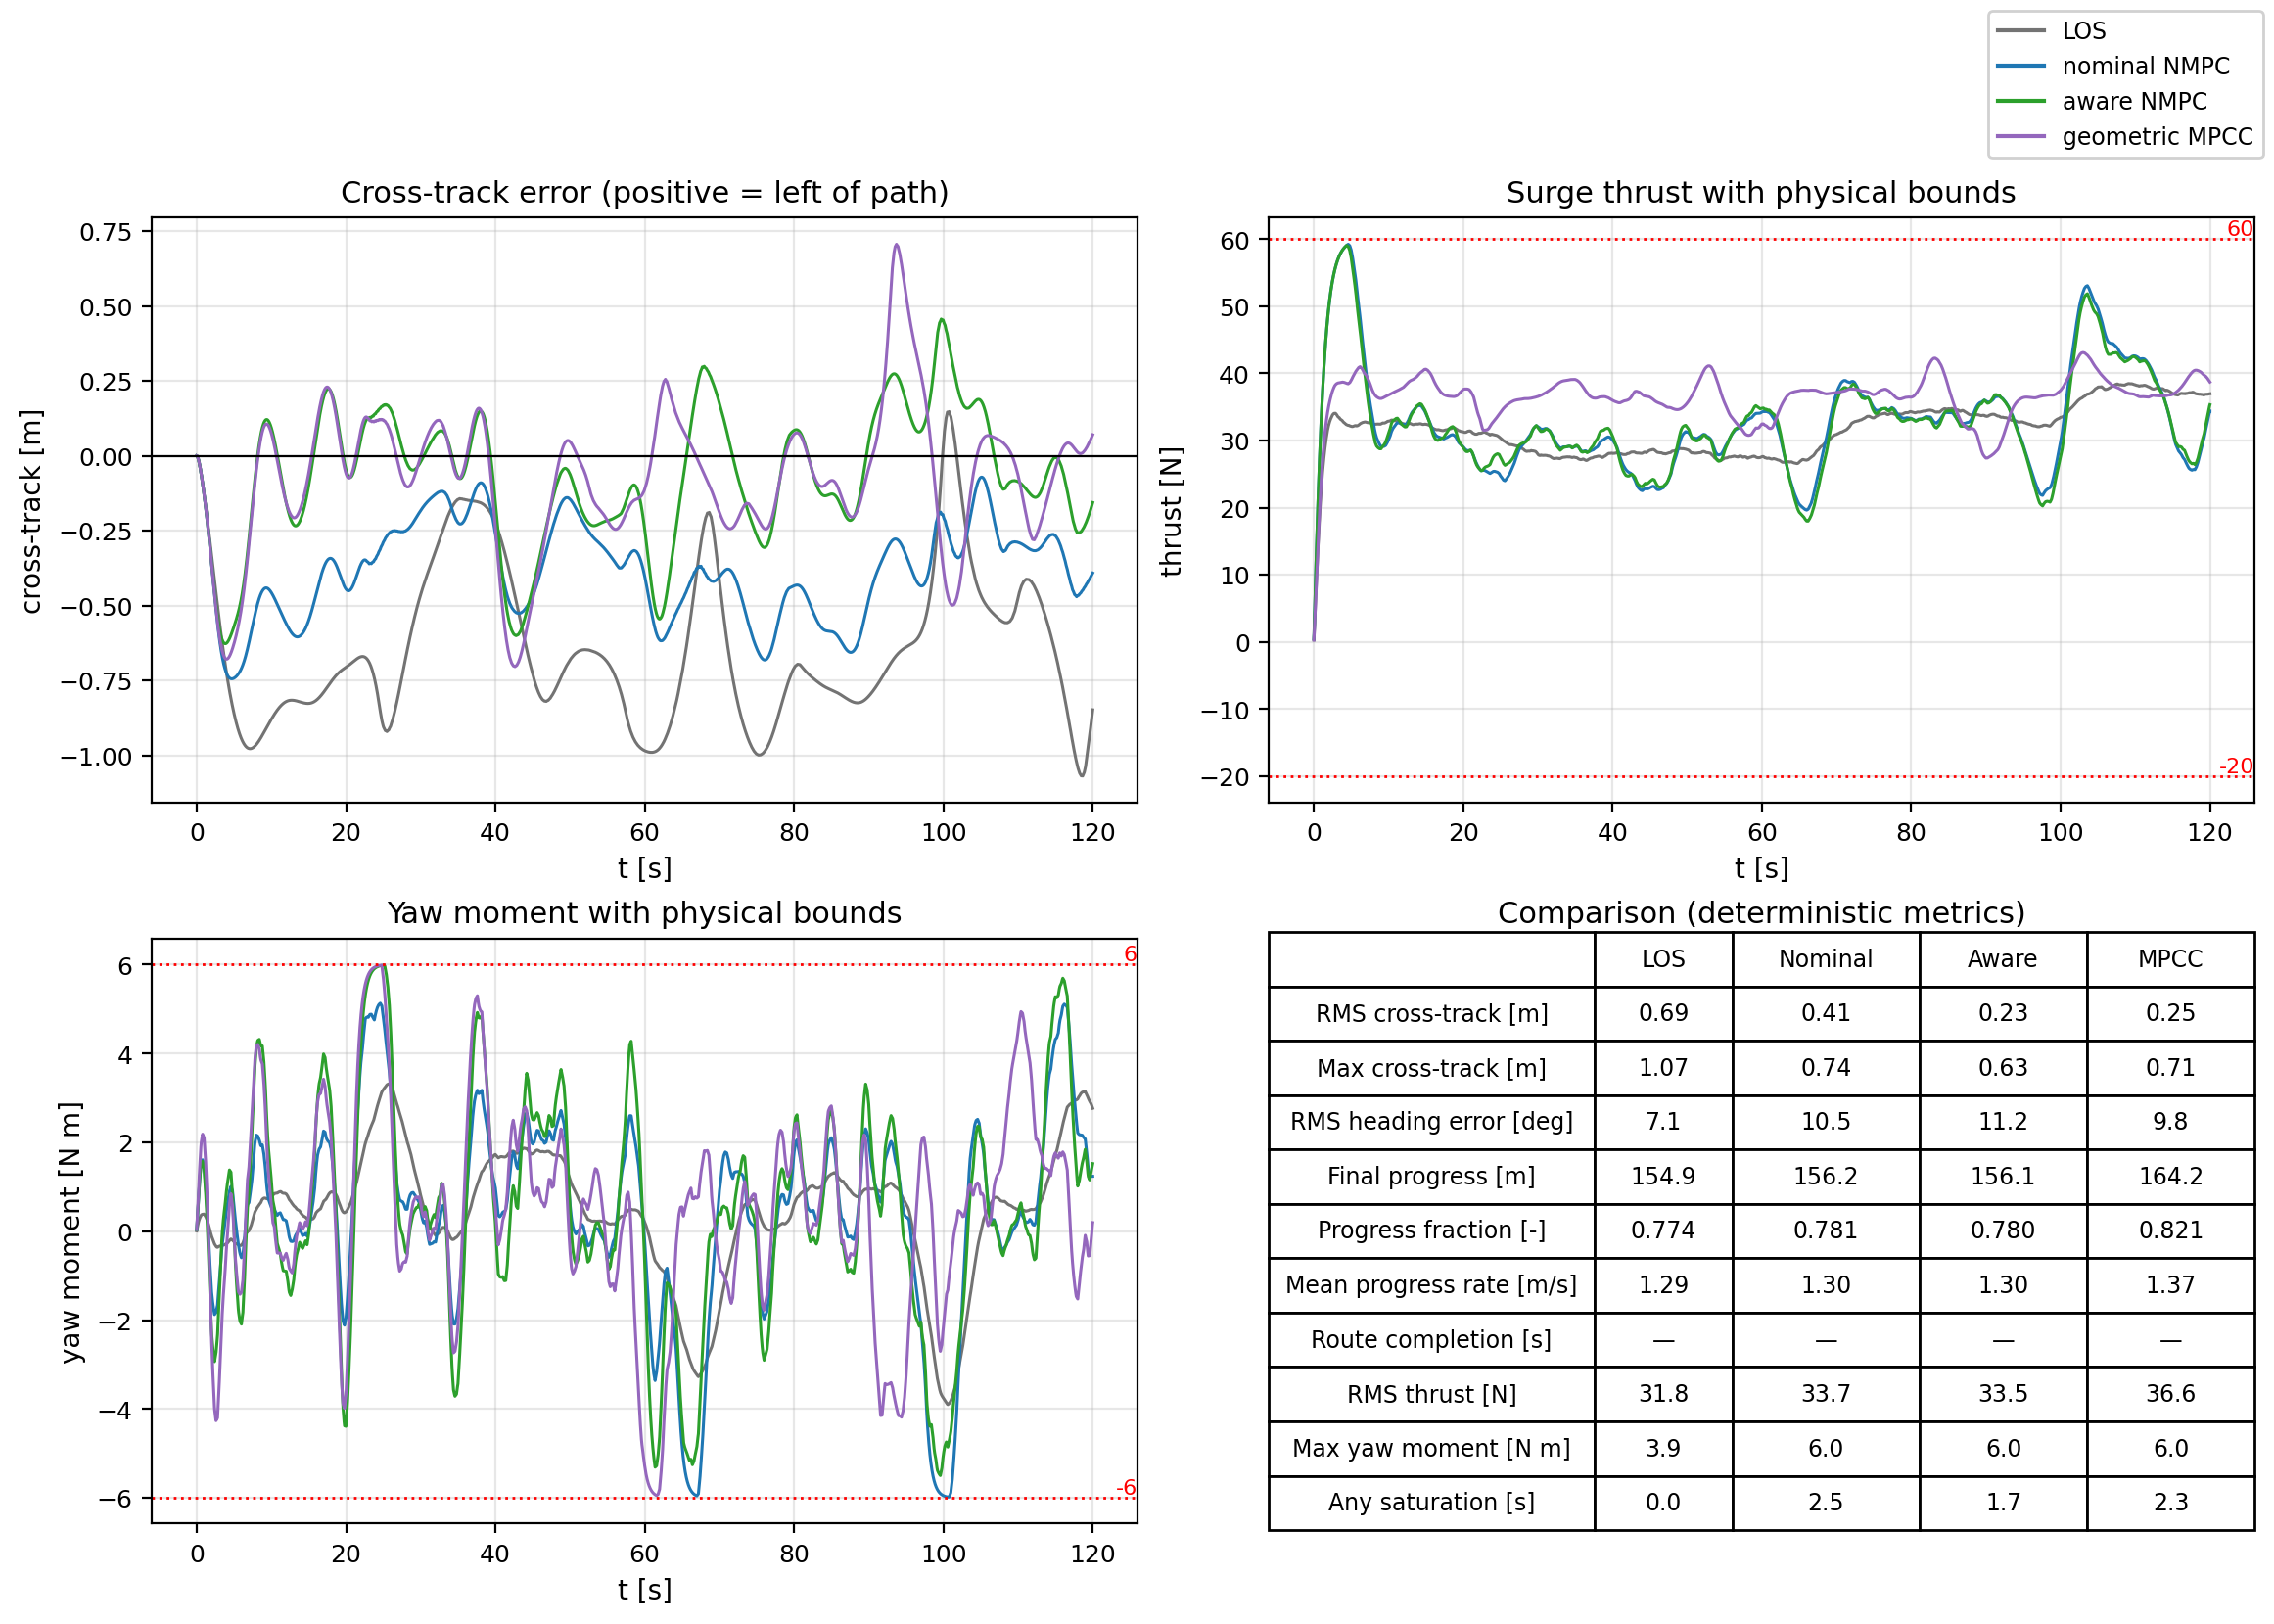
\includegraphics[width=0.98\textwidth]{figs/controller_comparison.png}
  \caption{Cross-track error, applied thrust and yaw moment with the
  physical bounds, and the deterministic metrics. The four controllers
  face the same estimator, the same perturbed plant and the same
  disturbances.}
  \label{fig:comparison}
\end{figure}

Mean solve times on this workload are 20.1\,ms (nominal NMPC), 16.7\,ms
(disturbance-aware NMPC) and 27.5\,ms (MPCC), against a 200\,ms budget at
5\,Hz. These are wall-clock measurements of a workload, kept strictly
apart from the deterministic metrics; no real-time capability is claimed.

\section{Reproducibility}
Every public number is produced by one tool from one reference run and
written to committed JSON artifacts (scenario configuration, deterministic
metrics, benchmark timings, software provenance). A content fingerprint of
the source tree binds the artifacts to the code that produced them;
\texttt{--check} validates schema, fingerprint, hashes and the generated
documentation tables without simulating anything, and
\texttt{--verify-determinism} replays the full flagship and compares it
against the committed metrics (LOS exactly, solver-based metrics within
$10^{-6}$ relative). Canonical generation pins single-threaded BLAS, since
threaded factorizations can flip the last ulps of an IPOPT iterate and
with it the accepted status of a borderline solve.

\section{Limitations and outlook}
The parameter set is illustrative (a $\sim$1.5\,m, 30\,kg USV,
order-of-magnitude values) and is not identified from a real hull; the
model is 3-DOF with no waves, no actuator dynamics beyond the rate limits,
and a uniform irrotational current. What the repository demonstrates is
the chain and its numerics, not vessel-specific fidelity. Planned work:
Monte-Carlo comparison of LOS against nominal and robust NMPC, and a
coastal environment for the flagship visual.

\begin{thebibliography}{9}
\bibitem{fossen2011}
T.~I. Fossen, \emph{Handbook of Marine Craft Hydrodynamics and Motion
Control}, Wiley, 2011.

\bibitem{fossen2002}
T.~I. Fossen, \emph{Marine Control Systems: Guidance, Navigation, and
Control of Ships, Rigs and Underwater Vehicles}, Marine Cybernetics, 2002.

\bibitem{mayne2000}
D.~Q. Mayne, J.~B. Rawlings, C.~V. Rao and P.~O.~M. Scokaert,
``Constrained model predictive control: Stability and optimality,''
\emph{Automatica}, 36(6), 2000.

\bibitem{kalman1960}
R.~E. Kalman, ``A new approach to linear filtering and prediction
problems,'' \emph{ASME Journal of Basic Engineering}, 82(1), 1960.

\bibitem{waechter2006}
A.~W\"achter and L.~T. Biegler, ``On the implementation of an
interior-point filter line-search algorithm for large-scale nonlinear
programming,'' \emph{Mathematical Programming}, 106(1), 2006.

\bibitem{andersson2019}
J.~A.~E. Andersson, J.~Gillis, G. Horn, J.~B. Rawlings and M. Diehl,
``CasADi: a software framework for nonlinear optimization and optimal
control,'' \emph{Mathematical Programming Computation}, 11(1), 2019.
\end{thebibliography}

\end{document}
